\documentclass{article}
\usepackage[utf8]{inputenc}
\usepackage[margin=1in]{geometry}
\usepackage{float}
\usepackage{tikz}
\usepackage{tikz-qtree}

\title{Data Structures: Problem Set 3}
\author{Jackie Luo}
\date{April 3, 2015}

\begin{document}
\maketitle

\section{Theory}

\subsection{}

\begin{figure}[H]
\centering
\begin{tikzpicture}
\Tree [.2 ]
\end{tikzpicture}
\caption{Tree is balanced, no rotation required}
\end{figure}

\begin{figure}[H]
\centering
\begin{tikzpicture}
\Tree [.2 1 \edge[draw=none]; {} ]
\end{tikzpicture}
\caption{Tree is balanced, no rotation required}
\end{figure}

\begin{figure}[H]
\centering
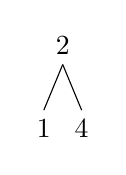
\begin{tikzpicture}
\Tree [.2 1 4 ]
\end{tikzpicture}
\caption{Tree is balanced, no rotation required}
\end{figure}

\begin{figure}[H]
\centering
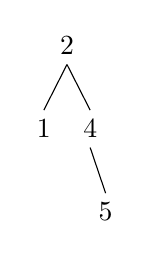
\begin{tikzpicture}
\Tree [.2 1 [.4 \edge[draw=none]; {} 5 ] ]
\end{tikzpicture}
\caption{Tree is balanced, no rotation required}
\end{figure}

\begin{figure}[H]
\centering
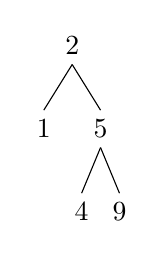
\begin{tikzpicture}
\Tree [.2 1 [.5 4 9 ] ]
\end{tikzpicture}
\caption{Rotated 4 to the left (single)}
\end{figure}

\begin{figure}[H]
\centering
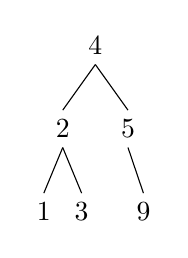
\begin{tikzpicture}
\Tree [.4 [.2 1 3 ] [.5 \edge[draw=none]; {} 9 ] ]
\end{tikzpicture}
\caption{Rotated 2 to the left (double)}
\end{figure}

\begin{figure}[H]
\centering
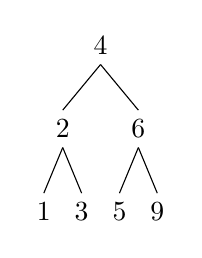
\begin{tikzpicture}
\Tree [.4 [.2 1 3 ] [.6 5 9 ] ]
\end{tikzpicture}
\caption{Rotated 5 to the left (single)}
\end{figure}

\begin{figure}[H]
\centering
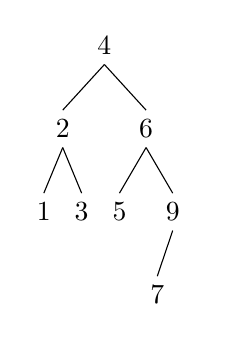
\begin{tikzpicture}
\Tree [.4 [.2 1 3 ] [.6 5 [.9 7 \edge[draw=none]; {} ] ] ]
\end{tikzpicture}
\caption{Tree is balanced, no rotation required}
\end{figure}

\subsection{}
To verify that the height information of an AVL tree is correctly maintained and that the balance property is in order, you can traverse the tree through a node's children with the following pseudocode: \vspace{5mm}
\newline
height(node):
\newline
\indent if node is null:
\newline
\indent \indent return -1
\newline
\indent else:
\newline
\indent \indent return max(height(node.left), height(node.right)) + 1 \vspace{5mm}
\newline
If the absolute value of the difference between a node's left and right children is ever greater than or equal to 2, then the algorithm can return "false." If all of the nodes are reached and the heights for the children have a difference of 1 or 0, then the algorithm returns "true."

\subsection{}
Separate Chaining
\newline
$0
\newline
1 \rightarrow 4371
\newline
2
\newline
3 \rightarrow 1323 \rightarrow 6173
\newline
4 \rightarrow 4344
\newline
5
\newline
6
\newline
7
\newline
8
\newline
\vspace{5mm} 9 \rightarrow 4199 \rightarrow 9679 \rightarrow 1989$

\noindent Quadratic Probing
\newline
$0: 9679
\newline
1: 4371
\newline
2
\newline
3: 1323
\newline
4: 6173
\newline
5: 4344
\newline
6
\newline
7
\newline
8: 1989
\newline
\vspace{5mm} 9: 4199$

\noindent Double Hashing
\newline
$hash_2(x) = 8 - x % 4
\newline
0: 6173
\newline
1: 4371
\newline
2
\newline
3: 1323
\newline
4: 4344
\newline
5: 9679
\newline
6: 1989
\newline
7
\newline
8
\newline
9: 4199$

\subsection{}
To compute a hash value for a binary tree, you could use in-order traversal to get the value of each node (recursively for the left child, then for the right). At the same time, keep track of the index of the node. For instance, the root node could be 1, the left child could be 2, and so on. That would help ensure that binary trees with the same values in different structures would have different hash values, since the nodes' orders in the in-order traversal would differ, so their indexes would differ. The hash value for the node could be calculated by the value of the node times the index (i.e., (12 * 4) mod 7 for a node with a value of 12 in the fourth position of the in-order traversal and a hash function of $x$ mod 7. For the whole binary tree, you could add all of the nodes' hash values.

\end{document}